\section{Utente Autenticato}

Di seguito vengono elencati i casi d'uso per l'utente autenticato.
\subsection{Casi d'Uso}

\subsubsection{UC-U8}

    \begin{figure}[H]
      \begin{center}
        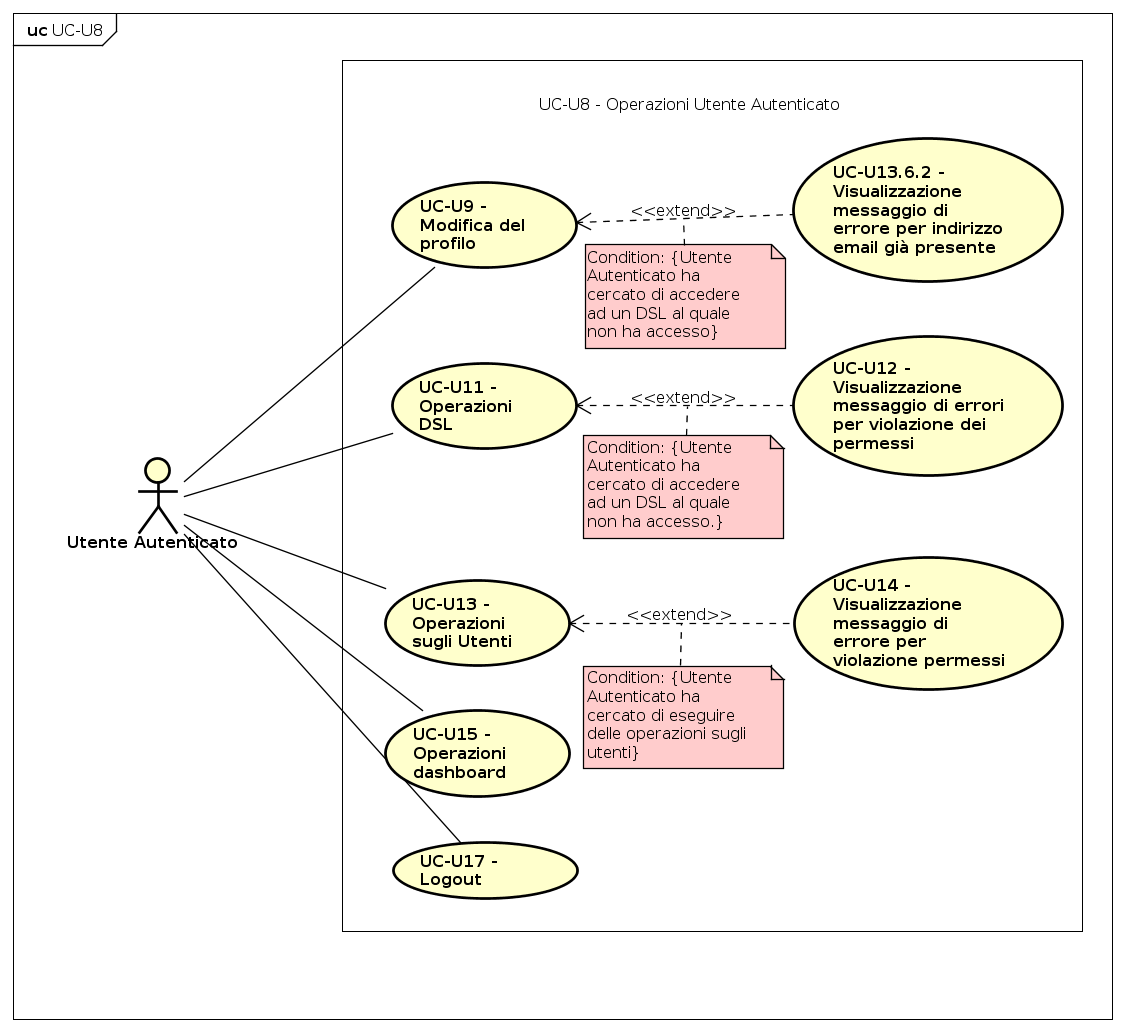
\includegraphics[width=12cm]{res/img/UCUtenti/UCUtenteA/UC-U8.png}
      \caption{UC-U8 - Operazioni dell'utente autenticato}
      \end{center} 
    \end{figure}    
    
    %Tabella 
    \begin{center}
      \bgroup
      \def\arraystretch{1.8}     
      \begin{longtable}{  p{3.5cm} | p{8cm} } 
        
        \hline
        \multicolumn{2}{ | c | }{ \cellcolor[gray]{0.9} \textbf{UC-U8 - Operazioni dell'utente autenticato}} \\ 
        \hline
        
        \textbf{Attori Primari} & Utente autenticato \\ 
        \textbf{Scopo e Descrizione} & L’utente autenticato può: modificare il proprio profilo, effettuare delle operazioni nella pagina \glossaryItem{Dashboard}, effettuare delle operazioni di creazione/modifica/esecuzione del DSL (a seconda dei suoi permessi) e gestire altri utenti (quest'ultima funzionalità è riservata ad un ruolo superiore o uguale all'admin). \\ 
        
        \textbf{Precondizioni}  & L’applicazione è funzionante e pronta all'uso. L'utente autenticato ha visualizzato la
        pagina \glossaryItem{Dashboard}. \\ 
        
        \textbf{Postcondizioni} & L'applicazione ha eseguito le azioni richieste dall'utente. \\ 
        \textbf{Scenario principale} & 1. L'utente modifica il proprio profilo. (UC-U9)
        
2. L'utente effettua delle operazioni nella pagina \glossaryItem{Dashboard}. (UC-U15)

3. L'utente effettua delle operazioni di creazione/modifica/esecuzione del DSL (a seconda dei suoi permessi). (UC-U11)

4. L'utente gestisce altri utenti (quest'ultima funzionalità è riservata ad un ruolo superiore o uguale all'admin). (UC-U13)

5. L'utente effettua il logout. (UC-U17) \\
        \textbf{Estensioni} & 1. L'utente autenticato visualizza un messaggio di errore nella procedura di modifica del profilo dovuto all'inserimento di un indirizzo email già presente (UC-U13.6.2)
        
2. L'utente autenticato visualizza un messaggio di errore durante le operazioni effettuate sul DSL dovuto alla violazione dei permessi. (UC-U12)

3. L'utente autenticato visualizza un messaggio di errore durante le operazioni sugli utenti dovute alla violazione dei permessi. (UC-u14) \\
      \end{longtable}
      \egroup
    \end{center} 


\subsubsection{UC-U9}

    \begin{figure}[H]
      \begin{center}
        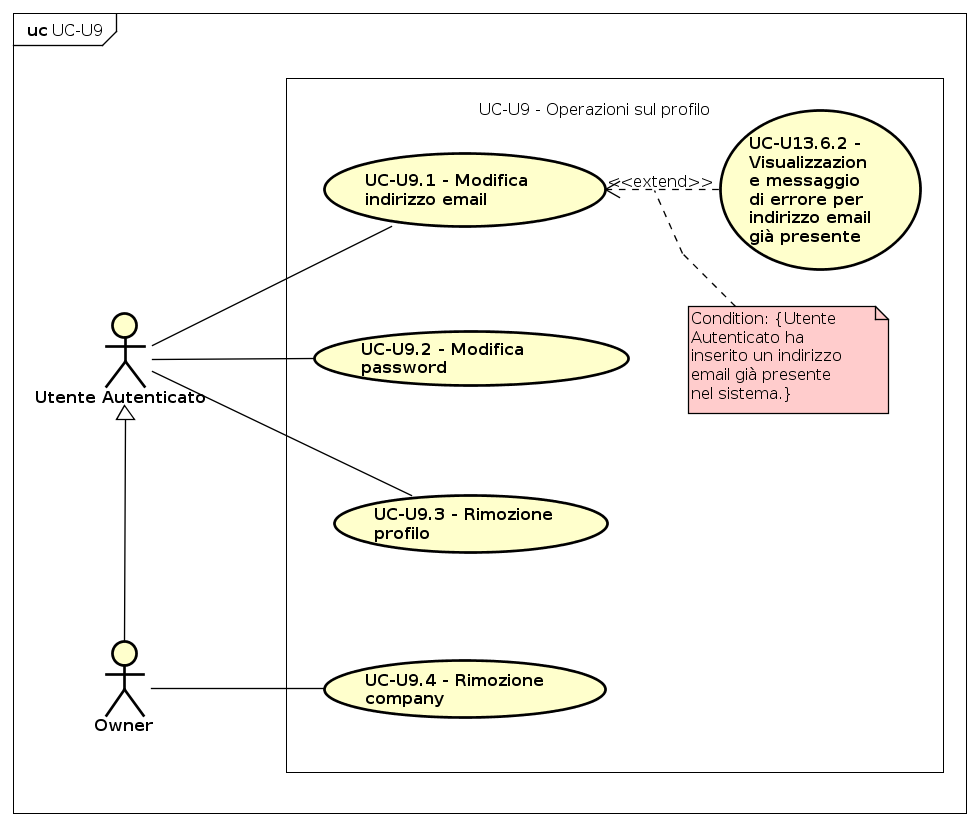
\includegraphics[width=12cm]{res/img/UCUtenti/UCUtenteA/UC-U9- Operazioni sul profilo/UC-U9.png}
      \caption{UC-U9 - Operazioni sul profilo}
      \end{center} 
    \end{figure}    
    
    %Tabella 
    \begin{center}
      \bgroup
      \def\arraystretch{1.8}     
      \begin{longtable}{  p{3.5cm} | p{8cm} } 
        
        \hline
        \multicolumn{2}{ | c | }{ \cellcolor[gray]{0.9} \textbf{UC-U9 - Operazioni sul profilo}} \\ 
        \hline
        
        \textbf{Attori Primari} & Utente autenticato \\ 
        \textbf{Scopo e Descrizione} & L'utente autenticato visualizza la pagina per apportare modifiche al profilo personale. Può decidere di: modificare l'indirizzo email, la password, o rimuovere il profilo. \\ 
        
        \textbf{Precondizioni}  & L’applicazione è funzionante e pronta all'uso. L'utente autenticato ha visualizzato la
        pagina \glossaryItem{Dashboard}. \\ 
        
        \textbf{Postcondizioni} & Le (eventuali) modifiche del profilo richieste dall'utente sono state apportate. \\ 
        \textbf{Scenario principale} & 1. L'utente autenticato modifica il proprio indirizzo email. (UC-U9.1)
        
2. L'utente autenticato modifica la propria password. (UC-U9.2)

3. L'utente autenticato rimuove il suo profilo/account. (UC-U9.3)

4. L'\textit{Owner} rimuove la propria \textit{Company} (UC-U9.4) \\
        \textbf{Estensioni} & 1. L'utente visualizza un messaggio di errore durante la modifica dell'email dovuto all'inserimento di un indirizzo email già presente. (UC-U13.6.2)  
      \end{longtable}
      \egroup
    \end{center} 

\subsubsection{UC-U9.1}
 

    \begin{figure}[H]
      \begin{center}
        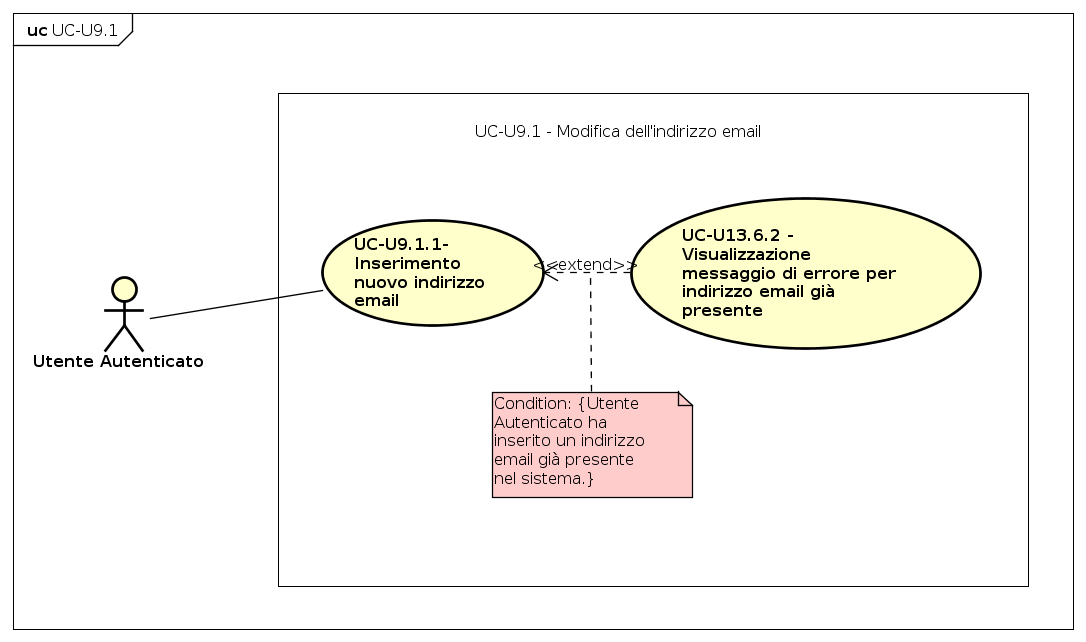
\includegraphics[width=12cm]{res/img/UCUtenti/UCUtenteA/UC-U9.1-Modifica indirizzo email/UC-U9.1.png}
      \caption{UC-U9.1 - Modifica indirizzo email}
      \end{center} 
    \end{figure}

    %Tabella 
    \begin{center}
      \bgroup
      \def\arraystretch{1.8}     
      \begin{longtable}{  p{3.5cm} | p{8cm} } 
        
        \hline
        \multicolumn{2}{ | c | }{ \cellcolor[gray]{0.9} \textbf{UC-U9.1 - Modifica indirizzo email}} \\ 
        \hline
        
        \textbf{Attori Primari} & Utente autenticato \\ 
        \textbf{Scopo e Descrizione} & L'utente autenticato può modificare il proprio indirizzo email nella procedura di modifica del profilo. \\ 
        
        \textbf{Precondizioni}  & L'utente autenticato ha visualizzato la pagina di modifica del profilo. \\ 
        
        \textbf{Postcondizioni} & Il sistema registra un nuovo indirizzo email per il profilo dell'attore. \\ 
        \textbf{Scenario principale} & 1. L'utente autenticato inserisce un nuovo indirizzo email. (UC-U9.1.1) \\
        \textbf{Estensioni} & 1. L'utente autenticato visualizza un messaggio di errore causato dall'inserimento di un indirizzo email già presente. (UC-U13.6.2) \\
      \end{longtable}
      \egroup
    \end{center}
    
\subsubsection{UC-U9.1.1}

    %Tabella 
    \begin{center}
      \bgroup
      \def\arraystretch{1.8}     
      \begin{longtable}{  p{3.5cm} | p{8cm} } 
        
        \hline
        \multicolumn{2}{ | c | }{ \cellcolor[gray]{0.9} \textbf{UC-U9.1.1 - Inserimento di un nuovo indirizzo email}} \\ 
        \hline
        
        \textbf{Attori Primari} & Utente autenticato \\ 
        \textbf{Scopo e Descrizione} & L'utente autenticato può inserire un nuovo indirizzo email nella procedura di modifica del profilo. \\ 
        
        \textbf{Precondizioni}  & L'utente autenticato ha visualizzato la pagina di modifica del profilo. \\ 
        
        \textbf{Postcondizioni} & L'utente autenticato ha inserito un nuovo indirizzo email. \\ 
      \end{longtable}
      \egroup
    \end{center}
    
    
\subsubsection{UC-U9.2}
 

    \begin{figure}[H]
      \begin{center}
        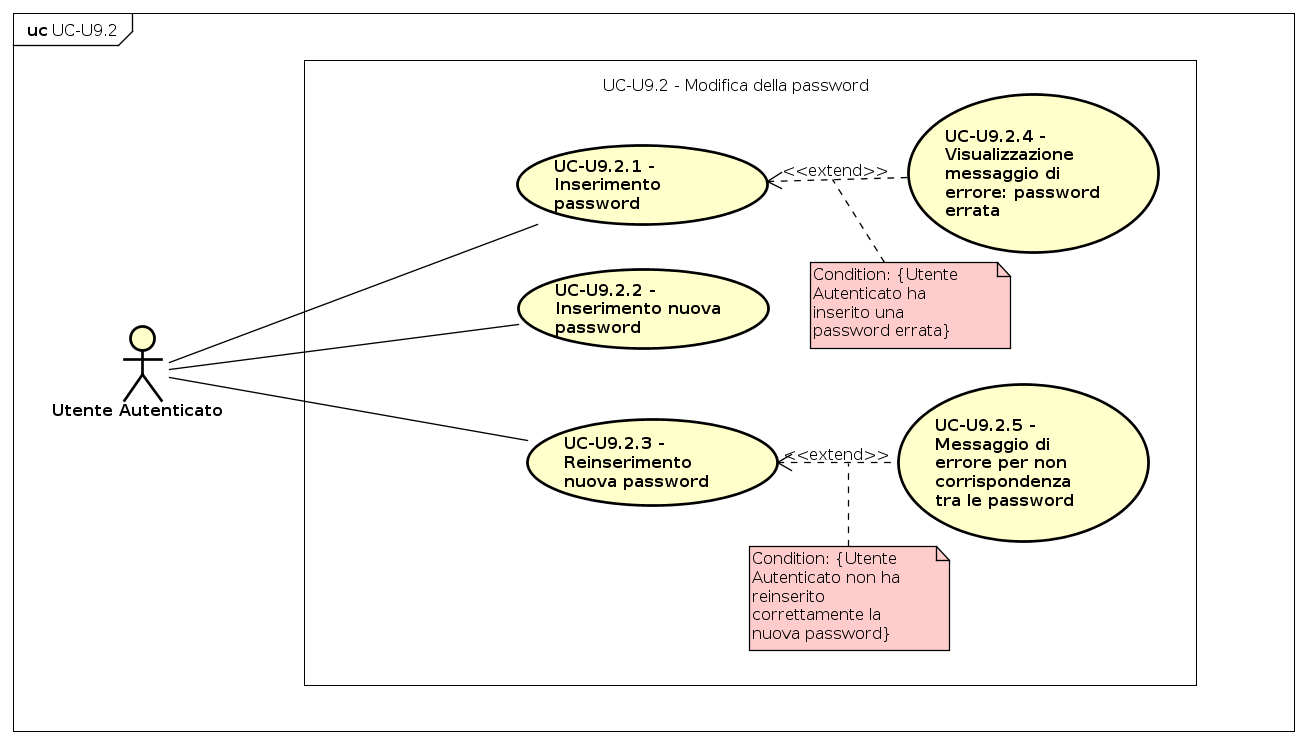
\includegraphics[width=12cm]{res/img/UCUtenti/UCUtenteA/UC-U9.2-Modifica password/UC-U9.2.png}
      \caption{UC-U9.2 - Modifica password}
      \end{center} 
    \end{figure}

    %Tabella 
    \begin{center}
      \bgroup
      \def\arraystretch{1.8}     
      \begin{longtable}{  p{3.5cm} | p{8cm} } 
        
        \hline
        \multicolumn{2}{ | c | }{ \cellcolor[gray]{0.9} \textbf{UC-U9.2 - Modifica password}} \\ 
        \hline
        
        \textbf{Attori Primari} & Utente autenticato \\ 
        \textbf{Scopo e Descrizione} & L'utente autenticato può modificare la password del proprio account. \\ 
        
        \textbf{Precondizioni}  & L'utente autenticato ha visualizzato la pagina di modifica del profilo. \\ 
        
        \textbf{Postcondizioni} & L'utente autenticato ha sostituito la password precedente con quella da lui inserita. \\ 
        \textbf{Scenario principale} & 1. L'utente autenticato inserisce la password corrente. (UC-U9.2.1)
        
2. L'utente autenticato inserisce una nuova password. (UC-U9.2.2)

3. L'utente autenticato re-inserisce la nuova password. (UC-U9.2.3) \\
        \textbf{Estensioni} & 1. L'utente autenticato visualizza un messaggio di errore dovuto all'inserimento di una password errata. (UC-U9.2.4)
        
2. L'attore visualizza un messaggio di errore causato dalla non corrispondenza tra le password inserite. (UC-U9.2.5) \\
      \end{longtable}
      \egroup
    \end{center}
    
\subsubsection{UC-U9.2.1}

    %Tabella 
    \begin{center}
      \bgroup
      \def\arraystretch{1.8}     
      \begin{longtable}{  p{3.5cm} | p{8cm} } 
        
        \hline
        \multicolumn{2}{ | c | }{ \cellcolor[gray]{0.9} \textbf{UC-U9.2.1 - Inserimento Password}} \\ 
        \hline
        
        \textbf{Attori Primari} & Utente autenticato \\ 
        \textbf{Scopo e Descrizione} & L'utente autenticato inserisce la propria password. \\ 
        
        \textbf{Precondizioni}  & L'utente autenticato ha visualizzato la pagina di modifica del profilo. \\ 
        
        \textbf{Postcondizioni} & L'utente autenticato ha inserito la propria password. \\ 
      \end{longtable}
      \egroup
    \end{center}
\subsubsection{UC-U9.2.2}

    %Tabella 
    \begin{center}
      \bgroup
      \def\arraystretch{1.8}     
      \begin{longtable}{  p{3.5cm} | p{8cm} } 
        
        \hline
        \multicolumn{2}{ | c | }{ \cellcolor[gray]{0.9} \textbf{UC-U9.2.2 - Inserimento nuova password}} \\ 
        \hline
        
        \textbf{Attori Primari} & Utente autenticato \\ 
        \textbf{Scopo e Descrizione} & L'utente autenticato inserisce una nuova password in sostituzione di quella precedente.  \\ 
        
        \textbf{Precondizioni}  & L'utente autenticato ha visualizzato la pagina di modifica del profilo. \\ 
        
        \textbf{Postcondizioni} & L'utente autenticato ha inserito una nuova password. \\ 
      \end{longtable}
      \egroup
    \end{center}
	
\subsubsection{UC-U9.2.3}

    %Tabella 
    \begin{center}
      \bgroup
      \def\arraystretch{1.8}     
      \begin{longtable}{  p{3.5cm} | p{8cm} } 
        
        \hline
        \multicolumn{2}{ | c | }{ \cellcolor[gray]{0.9} \textbf{UC-U9.2.3 - Reinserimento password}} \\ 
        \hline
        
        \textbf{Attori Primari} & Utente autenticato \\ 
        \textbf{Scopo e Descrizione} & L'utente autenticato ripete l'inserimento della nuova password. \\ 
        
        \textbf{Precondizioni}  & L'utente autenticato ha precedentemente inserito la nuova password. (UC-U9.2.2) \\ 
        
        \textbf{Postcondizioni} & L'utente autenticato ha completato la procedura di cambiamento della password. La nuova password inserita ha sostituito la password precedente. \\ 
      \end{longtable}
      \egroup
    \end{center}

\subsubsection{UC-U9.2.4}

    %Tabella 
    \begin{center}
      \bgroup
      \def\arraystretch{1.8}     
      \begin{longtable}{  p{3.5cm} | p{8cm} } 
        
        \hline
        \multicolumn{2}{ | c | }{ \cellcolor[gray]{0.9} \textbf{UC-U9.2.4 - Visualizzazione messaggio di errore: password errata}} \\ 
        \hline
        
        \textbf{Attori Primari} & Utente autenticato \\ 
        \textbf{Scopo e Descrizione} & L'utente autenticato visualizza un messaggio di errore durante procedura di modifica del profilo dovuto all'inserimento di una password errata. \\ 
        
        \textbf{Precondizioni}  & L'utente autenticato ha inserito una password errata nella procedura di cambio della password. \\ 
        
        \textbf{Postcondizioni} & L'utente autenticato ha visualizzato il messaggio di errore. \\ 
      \end{longtable}
      \egroup
    \end{center}

\subsubsection{UC-U9.2.5}

    %Tabella 
    \begin{center}
      \bgroup
      \def\arraystretch{1.8}     
      \begin{longtable}{  p{3.5cm} | p{8cm} } 
        
        \hline
        \multicolumn{2}{ | c | }{ \cellcolor[gray]{0.9} \textbf{UC-U9.2.5 - Messaggio di errore per non corrispondenza tra le password}} \\ 
        \hline
        
        \textbf{Attori Primari} & Utente autenticato \\ 
        \textbf{Scopo e Descrizione} & L'utente autenticato visualizza un messaggio di errore dovuto al reinserimento errato della nuova password (la nuova password è diversa da quella inserita la prima volta). \\ 
        
        \textbf{Precondizioni}  & L'utente autenticato non ha reinserito correttamente la nuova password. \\ 
        
        \textbf{Postcondizioni} & L'utente autenticato ha visualizzato il messaggio di errore. \\ 
      \end{longtable}
      \egroup
    \end{center}
\subsubsection{UC-U9.3}

    %Tabella 
    \begin{center}
      \bgroup
      \def\arraystretch{1.8}     
      \begin{longtable}{  p{3.5cm} | p{8cm} } 
        
        \hline
        \multicolumn{2}{ | c | }{ \cellcolor[gray]{0.9} \textbf{UC-U9.3 - Rimozione profilo}} \\ 
        \hline
        
        \textbf{Attori Primari} & Utente autenticato \\ 
        \textbf{Scopo e Descrizione} & L'utente autenticato decide di rimuovere il suo profilo. \\ 
        
        \textbf{Precondizioni}  & L'utente autenticato ha acconsentito con la continuazione della procedura. \\ 
        
        \textbf{Postcondizioni} & L'utente autenticato visualizza un messaggio di avvenuta cancellazione e le sue credenziali vengono eliminate da MaaS. \\ 
      \end{longtable}
      \egroup
    \end{center}
\subsubsection{UC-U9.4}

    %Tabella 
    \begin{center}
      \bgroup
      \def\arraystretch{1.8}     
      \begin{longtable}{  p{3.5cm} | p{8cm} } 
        
        \hline
        \multicolumn{2}{ | c | }{ \cellcolor[gray]{0.9} \textbf{UC-U9.4 - Rimozione \glossaryItem{Company}}} \\ 
        \hline
        
        \textbf{Attori Primari} & \glossaryItem{Owner} \\ 
        \textbf{Scopo e Descrizione} & L'\glossaryItem{Owner} decide di rimuovere la \glossaryItem{Company} con tutte le sue informazioni e i suoi utenti. \\ 
        
        \textbf{Precondizioni}  & L'\glossaryItem{Owner} ha acconsentito alla continuazione della procedura. \\ 
        
        \textbf{Postcondizioni} & L'\glossaryItem{Owner} visualizza un messaggio di avvenuta cancellazione e tutti i dati e gli utenti collegati alla \glossaryItem{Company} vengono cancellati dal sistema. \\ 
      \end{longtable}
      \egroup
    \end{center}
\subsubsection{UC-U11}

        \begin{figure}[H]
          \begin{center}
            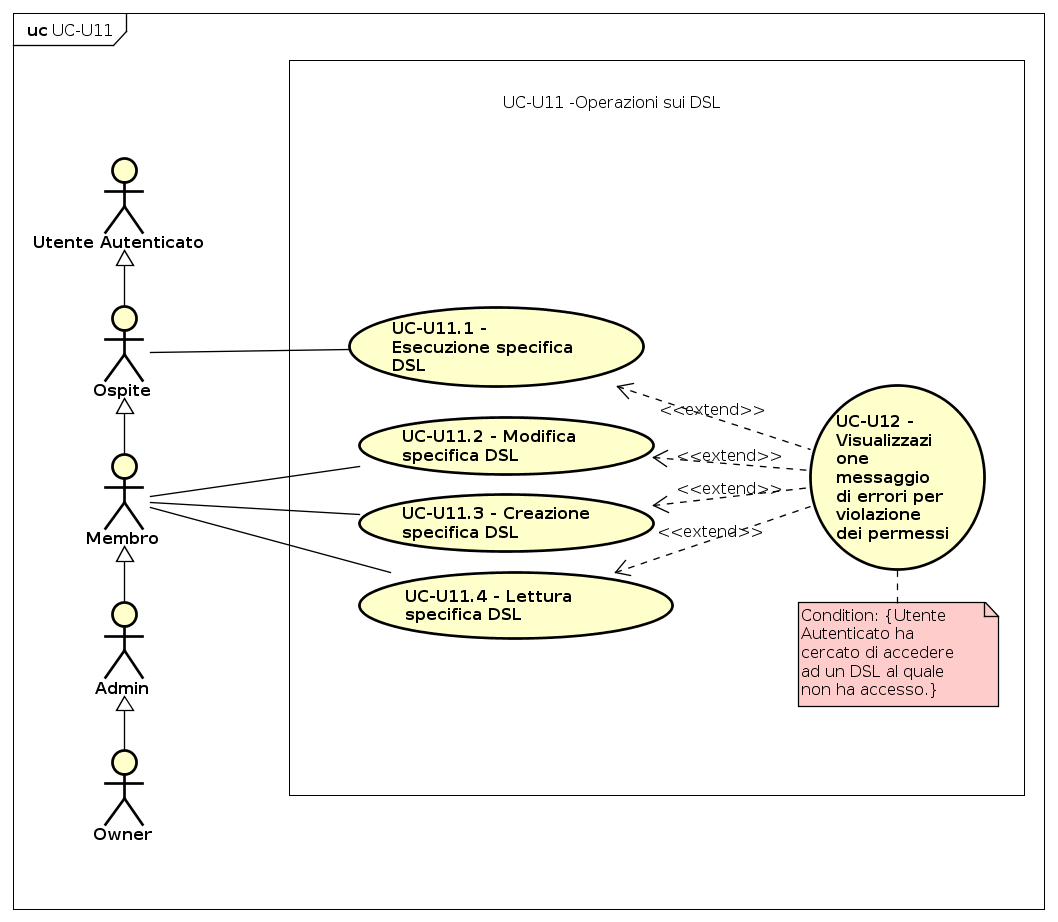
\includegraphics[width=12cm]{res/img/UCUtenti/UCUtenteA/UC-U11-Operazioni DSL/UC-U11.png}
          \caption{UC-U11 - Operazioni DSL}
          \end{center} 
        \end{figure}
        
        %Tabella 
        \begin{center}
          \bgroup
          \def\arraystretch{1.8}     
          \begin{longtable}{  p{3.5cm} | p{8cm} } 
            
            \hline
            \multicolumn{2}{ | c | }{ \cellcolor[gray]{0.9} \textbf{UC-U11 - Operazioni DSL}} \\ 
            \hline
            
            \textbf{Attori Primari} & Utente Autenticato, Ospite, Membro, Admin, \glossaryItem{Owner} \\ 
            \textbf{Scopo e Descrizione} & L’utente visualizza la pagina per apportare modifiche sulle DSL. Può decidere di: eseguire, modificare, creare e leggere una specifica DSL.\\ 
            
            \textbf{Precondizioni}  & L’applicazione MaaS è funzionante e pronta all'uso. Gli utenti possono accedere alla propria pagina \glossaryItem{Dashboard}. \\ 
            
            \textbf{Postcondizioni} & Le (eventuali) modifiche sono state apportate. \\ 
            \textbf{Scenario principale} & 1. L'Ospite, il Membro, l'Admin e l'\glossaryItem{Owner} possono eseguire una specifica DSL (UC-U11.1)  
            
            2. Il Membro, l'Admin e l'\textit{Owner} possono modificare una specifica DSL (UC-U11.2)
            
            3. Il Membro, l'Admin e l'\glossaryItem{Owner} possono creare una specifica DSL (UC-U11.3)
            
            4. Il Membro, l'Admin e l'\textit{Owner} possono leggere una specifica DSL (UC-U11.4)\\
            \textbf{Estensioni} & 1. L'utente visualizza un messaggio di errore in quanto non ha i permessi per operare sulla specifica DSL (UC-U12)  \\
          \end{longtable}
          \egroup
        \end{center}
\subsubsection{UC-U11.1}
                %Tabella 
                \begin{center}
                  \bgroup
                  \def\arraystretch{1.8}     
                  \begin{longtable}{  p{3.5cm} | p{8cm} } 
                    
                    \hline
                    \multicolumn{2}{ | c | }{ \cellcolor[gray]{0.9} \textbf{UC-U11.1 - Esecuzione specifica DSL}} \\ 
                    \hline
                    
                    \textbf{Attori Primari} & Utente Autenticato, Ospite, Membro, Admin, \textit{Owner}  \\ 
                    \textbf{Scopo e Descrizione} & L'Utente Autenticato, Ospite, Membro, Admin, \textit{Owner} eseguono una specifica DSL\\ 
                    
                    \textbf{Precondizioni}  & L’applicazione è funzionante e pronta all'uso. Gli utenti possono accedere alla propria pagina \glossaryItem{Dashboard}.\\ 
                    
                    \textbf{Postcondizioni} & L'utente visualizza il risultato della DSL \\ 
                    \textbf{Scenario principale} & Nessuno\\
                    \textbf{Estensioni} & 1. L'utente visualizza un messaggio di errore in quanto non ha i permessi per operare sulla specifica DSL (UC-U12)  \\
                  \end{longtable}
                  \egroup
                \end{center}
\subsubsection{UC-U11.2}
                %Tabella 
                \begin{center}
                  \bgroup
                  \def\arraystretch{1.8}     
                  \begin{longtable}{  p{3.5cm} | p{8cm} } 
                    
                    \hline
                    \multicolumn{2}{ | c | }{ \cellcolor[gray]{0.9} \textbf{UC-U11.2 - Modifica specifica DSL}} \\ 
                    \hline
                    
                    \textbf{Attori Primari} & Membro, Admin, \textit{Owner}  \\ 
                    \textbf{Scopo e Descrizione} & Il Membro, Admin, \textit{Owner} modificano una specifica DSL tramite l'editor\\ 
                    
                    \textbf{Precondizioni}  & L’applicazione è funzionante e pronta all'uso. Gli utenti possono accedere alla propria \glossaryItem{Dashboard}. \\ 
                    
                    \textbf{Postcondizioni} & L'utente modifica la DSL \\ 
                    \textbf{Estensioni} & 1. L'utente visualizza un messaggio di errore in quanto non ha i permessi per operare sulla specifica DSL (UC-U12)  \\
                  \end{longtable}
                  \egroup
                \end{center}
\subsubsection{UC-U11.3}
                %Tabella 
                \begin{center}
                  \bgroup
                  \def\arraystretch{1.8}     
                  \begin{longtable}{  p{3.5cm} | p{8cm} } 
                    
                    \hline
                    \multicolumn{2}{ | c | }{ \cellcolor[gray]{0.9} \textbf{UC-U11.3 - Creazione specifica DSL}} \\ 
                    \hline
                    
                    \textbf{Attori Primari} & Membro, Admin, \textit{Owner}  \\ 
                    \textbf{Scopo e Descrizione} & Il Membro, Admin, \textit{Owner} creano una specifica DSL tramite l'editor\\ 
                    
                    \textbf{Precondizioni}  & L’applicazione è funzionante e pronta all'uso. Gli utenti possono accedere alla propria pagina \glossaryItem{Dashboard}.\\ 
                    
                    \textbf{Postcondizioni} & L'utente aggiunge la DSL a MaaS \\ 
                    \textbf{Estensioni} & 1. L'utente visualizza un messaggio di errore in quanto non ha i permessi per operare sulla specifica DSL (UC-U12)  \\
                  \end{longtable}
                  \egroup
                \end{center}
\subsubsection{UC-U11.4}
                %Tabella 
                \begin{center}
                  \bgroup
                  \def\arraystretch{1.8}     
                  \begin{longtable}{  p{3.5cm} | p{8cm} } 
                    
                    \hline
                    \multicolumn{2}{ | c | }{ \cellcolor[gray]{0.9} \textbf{UC-U11.4 - Lettura specifica DSL}} \\ 
                    \hline
                    
                    \textbf{Attori Primari} & Membro, Admin, \textit{Owner}  \\ 
                    \textbf{Scopo e Descrizione} & Il Membro, Admin, \textit{Owner} leggono una specifica DSL\\ 
                    
                    \textbf{Precondizioni}  & L’applicazione è funzionante e pronta all'uso. Gli utenti possono accedere alla propria pagina \glossaryItem{Dashboard}.\\ 
                    
                    \textbf{Postcondizioni} & L'utente legge la DSL \\ 
                    \textbf{Estensioni} & 1. L'utente visualizza un messaggio di errore in quanto non ha i permessi per operare sulla specifica DSL (UC-U12)  \\
                  \end{longtable}
                  \egroup
                \end{center}
                
                
\subsubsection{UC-U12}
      
        %Tabella 
        \begin{center}
          \bgroup
          \def\arraystretch{1.8}     
          \begin{longtable}{  p{3.5cm} | p{8cm} } 
            
            \hline
            \multicolumn{2}{ | c | }{ \cellcolor[gray]{0.9} \textbf{UC-U12 - Visualizzazione di messaggio di errore per violazione dei permessi}} \\ 
            \hline
            
            \textbf{Attori Primari} & Utente autenticato \\ 
            \textbf{Scopo e Descrizione} & L’utente autenticato visualizza un messaggio di errore nel tentativo di eseguire un'operazione sul DSL.\\ 
            
            \textbf{Precondizioni}  & L'utente autenticato ha eseguito un'operazione sul DSL di cui non dispone i permessi. \\ 
            
            \textbf{Postcondizioni} & L'utente autenticato ha visualizzato il messaggio di errore. \\ 
          \end{longtable}
          \egroup
        \end{center}
\subsubsection{UC-U13}

        \begin{figure}[H]
          \begin{center}
            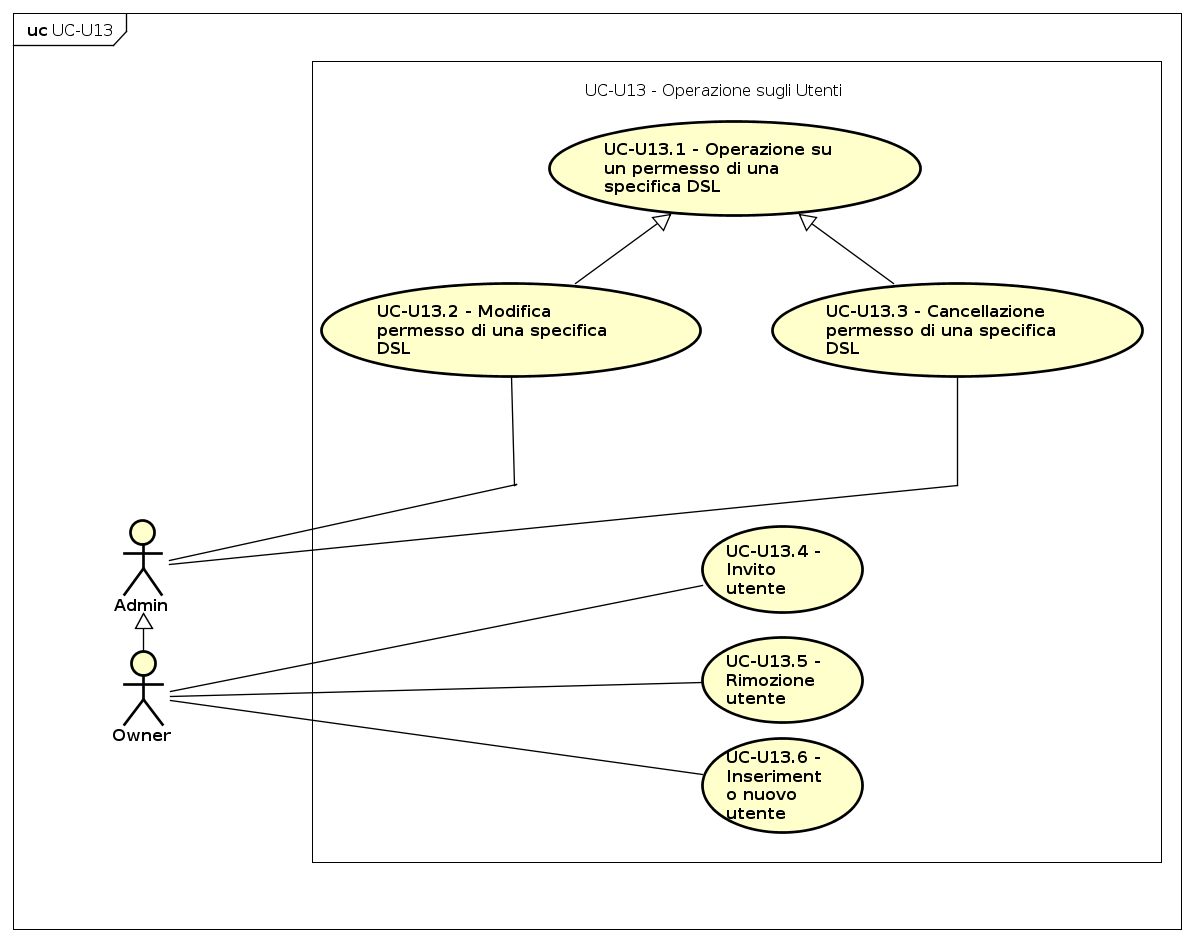
\includegraphics[width=12cm]{res/img/UCUtenti/UCUtenteA/UC-U13-Operazioni sugli Utenti/UC-U13.png}
          \caption{UC-U13 - Operazioni sugli utenti}
          \end{center} 
        \end{figure}
        
        %Tabella 
        \begin{center}
          \bgroup
          \def\arraystretch{1.8}     
          \begin{longtable}{  p{3.5cm} | p{8cm} } 
            
            \hline
            \multicolumn{2}{ | c | }{ \cellcolor[gray]{0.9} \textbf{UC-U13 - Operazioni sugli utenti}} \\ 
            \hline
            
            \textbf{Attori Primari} & Admin, \glossaryItem{Owner} \\ 
            \textbf{Scopo e Descrizione} & L'Admin e l'\glossaryItem{Owner} visualizzano la pagina per apportare modifiche sugli utenti. Possono decidere di: operare su una specifica DSL accedendo all'editor oppure inserire, rimuovere, invitare un nuovo utente.\\ 
            
            \textbf{Precondizioni}  & L'Admin e l'\glossaryItem{Owner} dispongono dei permessi. \\ 
            
            \textbf{Postcondizioni} & Le (eventuali) modifiche sono state apportate. \\ 
            \textbf{Scenario principale} & 1. L'Admin e l'\glossaryItem{Owner} possono eseguire operazioni su una specifica DSL (UC-U13.1)  
            
            2. L'\glossaryItem{Owner} può invitare un nuovo utente (UC-U13.4)
            
            3. L'\glossaryItem{Owner} può rimuovere un utente (UC-U13.5)
            
            4. L'\glossaryItem{Owner} può aggiungere un nuovo utente (UC-U13.6)\\
          \end{longtable}
          \egroup
        \end{center}
\subsubsection{UC-U13.1}
                %Tabella 
                \begin{center}
                  \bgroup
                  \def\arraystretch{1.8}     
                  \begin{longtable}{  p{3.5cm} | p{8cm} } 
                    
                    \hline
                    \multicolumn{2}{ | c | }{ \cellcolor[gray]{0.9} \textbf{UC-U13.1 - Operazione su un permesso di una specifica DSL}} \\ 
                    \hline
                    
                    \textbf{Attori Primari} & Amministratore, \glossaryItem{Owner} \\ 
                    \textbf{Scopo e Descrizione} & L'amministratore o l'\glossaryItem{Owner} decidono di operare su una specifica DSL\\ 
                    
                    \textbf{Precondizioni}  & La DSL selezionata è già stata creata in precedenza. \\ 
                    
                    \textbf{Postcondizioni} & L'operazione sulla specifica DSL è apportata. \\ 
                  \end{longtable}
                  \egroup
                \end{center}
                
                
                
\subsubsection{UC-U13.2}
                %Tabella 
                \begin{center}
                  \bgroup
                  \def\arraystretch{1.8}     
                  \begin{longtable}{  p{3.5cm} | p{8cm} } 
                    
                    \hline
                    \multicolumn{2}{ | c | }{ \cellcolor[gray]{0.9} \textbf{UC-U13.2 - Modifica permesso di una specifica DSL}} \\ 
                    \hline
                    
                    \textbf{Attori Primari} & Amministratore, \textit{Owner} \\ 
                    \textbf{Scopo e Descrizione} & L'amministratore o l'\textit{Owner} decidono di modificare il permesso di una specifica DSL\\ 
                    
                    \textbf{Precondizioni}  & La DSL selezionata è già stata creata in precedenza. \\ 
                    
                    \textbf{Postcondizioni} & La modifica sui permessi di una specifica DSL è apportata. \\ 
                  \end{longtable}
                  \egroup
                \end{center}
                
                
                
\subsubsection{UC-U13.3}
                %Tabella 
                \begin{center}
                  \bgroup
                  \def\arraystretch{1.8}     
                  \begin{longtable}{  p{3.5cm} | p{8cm} } 
                    
                    \hline
                    \multicolumn{2}{ | c | }{ \cellcolor[gray]{0.9} \textbf{UC-U13.3 - Cancellazione permesso di una specifica DSL}} \\ 
                    \hline
                    
                    \textbf{Attori Primari} & Amministratore, \textit{Owner} \\ 
                    \textbf{Scopo e Descrizione} & L'amministratore o l'\textit{Owner} decidono di cancellare un permesso su una specifica DSL\\ 
                    
                    \textbf{Precondizioni}  & La DSL selezionata è già stata creata in precedenza. \\ 
                    
                    \textbf{Postcondizioni} & La cancellazione del permesso sulla specifica DSL è apportata. \\ 
                  \end{longtable}
                  \egroup
                \end{center}
\subsubsection{UC-U13.4}
                %Tabella 
                \begin{center}
                  \bgroup
                  \def\arraystretch{1.8}     
                  \begin{longtable}{  p{3.5cm} | p{8cm} } 
                    
                    \hline
                    \multicolumn{2}{ | c | }{ \cellcolor[gray]{0.9} \textbf{UC-U13.4 - Invito utente}} \\ 
                    \hline
                    
                    \textbf{Attori Primari} & \textit{Owner} \\ 
                    \textbf{Scopo e Descrizione} & L'\textit{Owner} inserisce l'indirizzo email dell'utente che vuole invitare\\ 
                    
                    \textbf{Precondizioni}  & Nessuna. \\     %%TODO: non-sense
                    
                    \textbf{Postcondizioni} & L'utente è stato invitato. \\ 
                  \end{longtable}
                  \egroup
                \end{center}
\subsubsection{UC-U13.5}
                %Tabella 
                \begin{center}
                  \bgroup
                  \def\arraystretch{1.8}     
                  \begin{longtable}{  p{3.5cm} | p{8cm} } 
                    
                    \hline
                    \multicolumn{2}{ | c | }{ \cellcolor[gray]{0.9} \textbf{UC-U13.5 - Rimozione utente}} \\ 
                    \hline
                    
                    \textbf{Attori Primari} & \textit{Owner} \\ 
                    \textbf{Scopo e Descrizione} & L'\textit{Owner} inserisce l'indirizzo email dell'utente che vuole rimuovere\\ 
                    
                    \textbf{Precondizioni}  & L'indirizzo email utente è presente in MaaS. \\ 
                    
                    \textbf{Postcondizioni} & L'utente è stato rimosso. \\ 
                  \end{longtable}
                  \egroup
                \end{center}
                
\subsubsection{UC-U13.6}
                %Tabella 
                \begin{center}
                  \bgroup
                  \def\arraystretch{1.8}     
                  \begin{longtable}{  p{3.5cm} | p{8cm} } 
                    
                    \hline
                    \multicolumn{2}{ | c | }{ \cellcolor[gray]{0.9} \textbf{UC-U13.6 - Inserimento nuovo utente}} \\ 
                    \hline
                    
                    \textbf{Attori Primari} & \textit{Owner} \\ 
                    \textbf{Scopo e Descrizione} & L'\textit{Owner} inserisce un nuovo utente all'applicazione.\\ 
                    
                    \textbf{Precondizioni}  & Nessuna \\ 
                    
                    \textbf{Postcondizioni} & Un nuovo utente \`e stato aggiunto a \glossaryItem{MaaS}. \\ 
                  \end{longtable}
                  \egroup
                \end{center}
                
                
\subsubsection{UC-U13.6.2}

    %Tabella 
    \begin{center}
      \bgroup
      \def\arraystretch{1.8}     
      \begin{longtable}{  p{3.5cm} | p{8cm} } 
        
        \hline
        \multicolumn{2}{ | c | }{ \cellcolor[gray]{0.9} \textbf{UC-U13.6.2 - Visualizzazione di messaggio di errore per indirizzo email già presente}} \\ 
        \hline
        
        \textbf{Attori Primari} & Utente autenticato \\ 
        \textbf{Scopo e Descrizione} & L'utente autenticato visualizza un messaggio di errore durante la procedura di modifica del profilo causato dall'inserimento di un indirizzo email già presente nel sistema. \\ 
        
        \textbf{Precondizioni}  & L'utente autenticato ha inserito un indirizzo email già presente nel sistema. \\ 
        
        \textbf{Postcondizioni} & L'utente autenticato ha visualizzato il messaggio di errore. \\ 
      \end{longtable}
      \egroup
    \end{center}
\subsubsection{UC-U14}
      
        %Tabella 
        \begin{center}
          \bgroup
          \def\arraystretch{1.8}     
          \begin{longtable}{  p{3.5cm} | p{8cm} } 
            
            \hline
            \multicolumn{2}{ | c | }{ \cellcolor[gray]{0.9} \textbf{UC-U14 - Visualizzazione di messaggio di errore per violazione dei permessi}} \\ 
            \hline
            
            \textbf{Attori Primari} & Utente autenticato \\ 
            \textbf{Scopo e Descrizione} & L’utente autenticato visualizza un messaggio di errore nel tentativo di eseguire un'operazione su un utente.\\ 
            
            \textbf{Precondizioni}  & L'utente autenticato ha eseguito un'operazione su un utente di cui non dispone i permessi. \\ 
            
            \textbf{Postcondizioni} & L'utente autenticato ha visualizzato il messaggio di errore. \\ 
          \end{longtable}
          \egroup
        \end{center}
\subsubsection{UC-U15}
 

    \begin{figure}[H]
      \begin{center}
        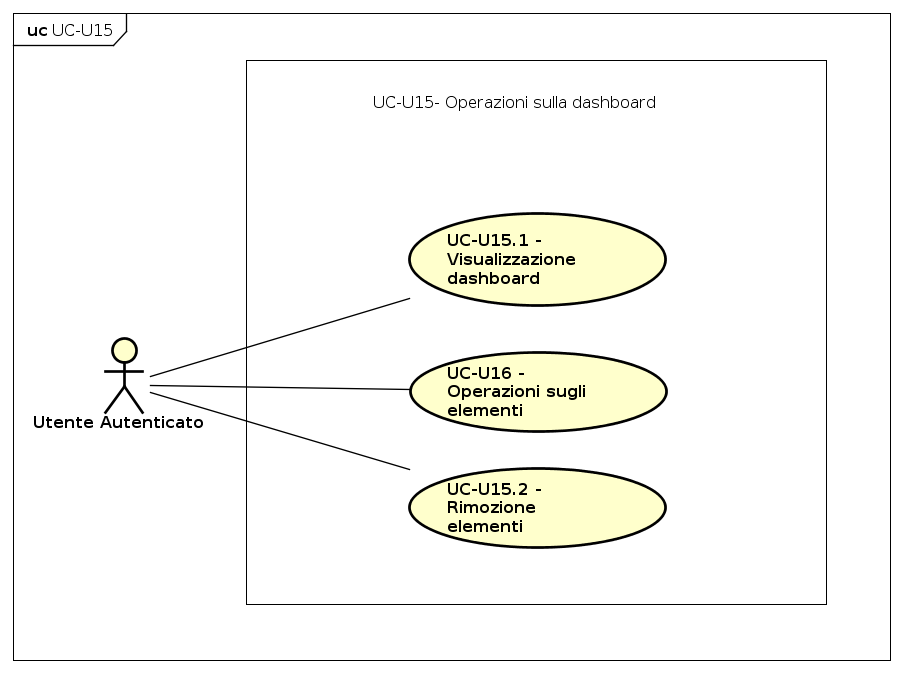
\includegraphics[width=12cm]{res/img/UCUtenti/UCUtenteA/UC-U15-Operazioni-dashboard/UC-U15.png}
      \caption{UC-U15 - Operazioni \glossaryItem{Dashboard}}
      \end{center} 
    \end{figure}

    %Tabella 
    \begin{center}
      \bgroup
      \def\arraystretch{1.8}     
      \begin{longtable}{  p{3.5cm} | p{8cm} } 
        
        \hline
        \multicolumn{2}{ | c | }{ \cellcolor[gray]{0.9} \textbf{UC-U15 - Operazioni \glossaryItem{Dashboard}}} \\ 
        \hline
        
        \textbf{Attori Primari} & Utente autenticato \\ 
        \textbf{Scopo e Descrizione} & L'utente autenticato può: visualizzare la \glossaryItem{Dashboard}, effettuare delle operazioni sulle righe della \glossaryItem{Dashboard}, rimuovere le righe della \glossaryItem{Dashboard}. \\ 
        
        \textbf{Precondizioni}  & L'utente autenticato si trova nella pagina iniziale \glossaryItem{Dashboard}. \\ 
        
        \textbf{Postcondizioni} & L'applicazione MaaS ha eseguito le operazioni richieste dall'utente. \\ 
        \textbf{Scenario principale} & 1. L'utente autenticato visualizza la \glossaryItem{Dashboard} (UC-U15.1)
        
2. L'utente autenticato effettua delle operazioni su un elemento della \glossaryItem{Dashboard} (UC-U16)

3. L'utente autenticato rimuove degli elementi dalla \glossaryItem{Dashboard} (UC-U15.2) \\
      \end{longtable}
      \egroup
    \end{center}

\subsubsection{UC-U15.1}

    %Tabella 
    \begin{center}
      \bgroup
      \def\arraystretch{1.8}     
      \begin{longtable}{  p{3.5cm} | p{8cm} } 
        
        \hline
        \multicolumn{2}{ | c | }{ \cellcolor[gray]{0.9} \textbf{UC-U15.1 - Visualizzazione \glossaryItem{Dashboard}}} \\ 
        \hline
        
        \textbf{Attori Primari} & Utente autenticato \\ 
        \textbf{Scopo e Descrizione} & L'utente autenticato visualizza la \glossaryItem{Dashboard}. \\ 
        
        \textbf{Precondizioni}  & L'applicazione mostra la \glossaryItem{Dashboard}. \\ 
        
        \textbf{Postcondizioni} & L'utente ha visualizzato la propria \glossaryItem{Dashboard}. \\ 
      \end{longtable}
      \egroup
    \end{center}
    
\subsubsection{UC-U15.2}

    %Tabella 
    \begin{center}
      \bgroup
      \def\arraystretch{1.8}     
      \begin{longtable}{  p{3.5cm} | p{8cm} } 
        
        \hline
        \multicolumn{2}{ | c | }{ \cellcolor[gray]{0.9} \textbf{UC-U15.2 - Rimozione elementi}} \\ 
        \hline
        
        \textbf{Attori Primari} & Utente autenticato \\ 
        \textbf{Scopo e Descrizione} & L'utente autenticato intende eliminare degli elementi presenti nella sua \glossaryItem{Dashboard}. \\ 
        
        \textbf{Precondizioni}  & L'utente si trova nella pagina \glossaryItem{Dashboard} e seleziona l'elemento che vuole eliminare. \\ 
        
        \textbf{Postcondizioni} & Il sistema ha rimosso l'elemento. \\ 
      \end{longtable}
      \egroup
    \end{center}

\subsubsection{UC-U16}

    \begin{figure}[H]
      \begin{center}
        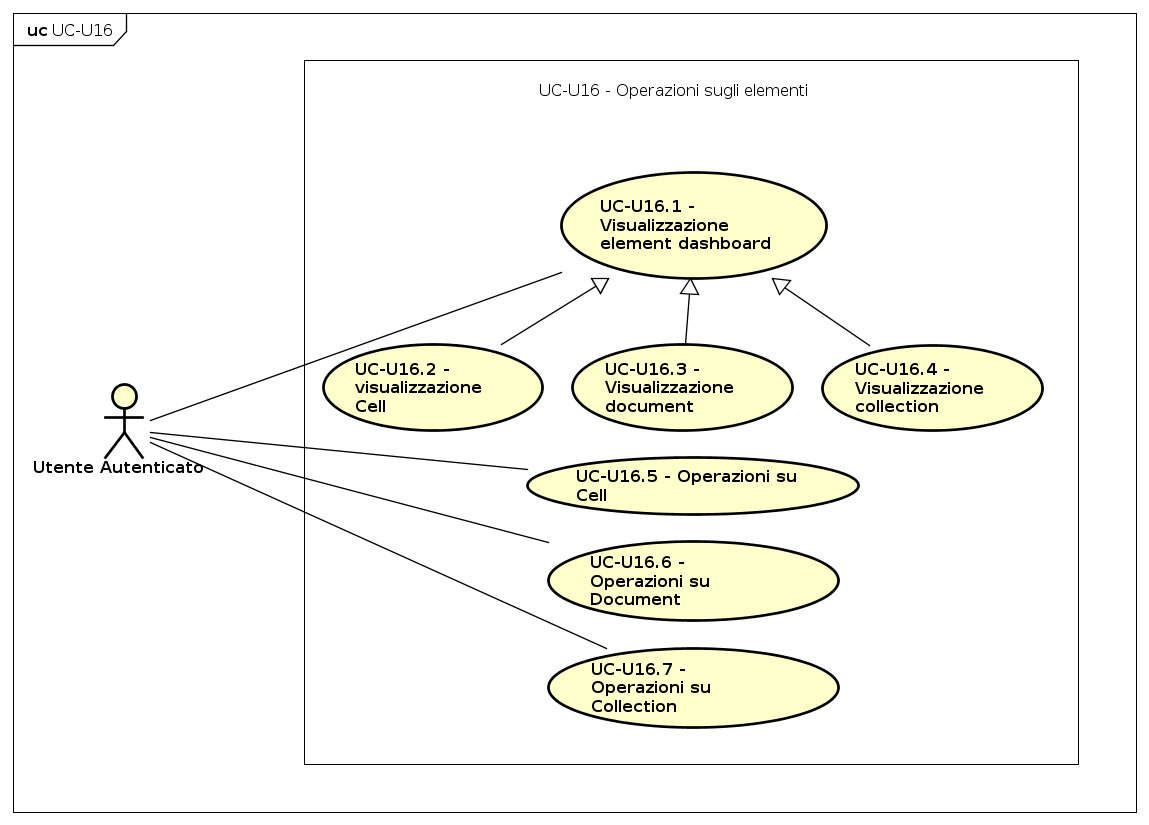
\includegraphics[width=12cm]{res/img/UCUtenti/UCUtenteA/UC-U16-Operazioni_sulle_righe/UC-U16.png}
      \caption{UC-U16 - Operazioni sugli elementi della \glossaryItem{Dashboard}}
      \end{center} 
    \end{figure}

    %Tabella 
    \begin{center}
      \bgroup
      \def\arraystretch{1.8}     
      \begin{longtable}{  p{3.5cm} | p{8cm} } 
        
        \hline
        \multicolumn{2}{ | c | }{ \cellcolor[gray]{0.9} \textbf{UC-U16 - Operazioni sugli elementi della \glossaryItem{Dashboard}}} \\ 
        \hline
        
        \textbf{Attori Primari} & Utente autenticato \\ 
        \textbf{Scopo e Descrizione} & L'utente autenticato può eseguire le seguenti azioni sugli elementi della \glossaryItem{Dashboard}: visualizzare un elemento (che può essere una \glossaryItem{Cell}, un \glossaryItem{Document} o una \glossaryItem{Collection}) oppure effettuare un'operazione su di esso. \\ 
        
        \textbf{Precondizioni}  & L'utente autenticato ha visualizzato la pagina iniziale \glossaryItem{Dashboard}. \\ 
        
        \textbf{Postcondizioni} & L'applicazione ha eseguito le operazioni sulle righe della \glossaryItem{Dashboard} richieste dall'utente autenticato. \\ 
        \textbf{Scenario principale} & 1. Visualizzazione element \glossaryItem{Dashboard} (UC-U16.1)
        
1.1 L'utente visualizza una \glossaryItem{Cell} (UC-U16.2)

1.2 L'utente visualizza un \glossaryItem{Document} (UC-U16.3)

1.3 L'utente visualizza una \glossaryItem{Collection} (UC-U16.4)

2. L'utente desidera effettuare un'operazione su una riga

2.1 L'utente effettua un'operazione su una \glossaryItem{Cell} (UC-U16.5)

2.2 L'utente effettua un'operazione su un \glossaryItem{Document} (UC-U16.6)

2.3 L'utente effettua un'operazione su una \glossaryItem{Collection} (UC-U16.7) \\
      \end{longtable}
      \egroup
    \end{center}
    
\subsubsection{UC-U16.1}

    %Tabella 
    \begin{center}
      \bgroup
      \def\arraystretch{1.8}     
      \begin{longtable}{  p{3.5cm} | p{8cm} } 
        
        \hline
        \multicolumn{2}{ | c | }{ \cellcolor[gray]{0.9} \textbf{UC-U16.1 - Visualizzazione element \glossaryItem{Dashboard}}} \\ 
        \hline
        
        \textbf{Attori Primari} & Utente autenticato \\ 
        \textbf{Scopo e Descrizione} & L'utente autenticato sceglie di visualizzare un element dalla \glossaryItem{Dashboard} (che può essere una \glossaryItem{Cell}, un \glossaryItem{Document} o una \glossaryItem{Collection}). \\ 
        
        \textbf{Precondizioni}  & L'utente autenticato ha visualizzato un element della \glossaryItem{Dashboard}. \\ 
        
        \textbf{Postcondizioni} & L'utente autenticato viene reindirizzato alla pagina di visione dell'element selezionato. \\ 
      \end{longtable}
      \egroup
    \end{center}

\newpage

\subsubsection{UC-U16.2}

    %Tabella 
    \begin{center}
      \bgroup
      \def\arraystretch{1.8}     
      \begin{longtable}{  p{3.5cm} | p{8cm} } 
        
        \hline
        \multicolumn{2}{ | c | }{ \cellcolor[gray]{0.9} \textbf{UC-U16.2 - Visualizzazione \glossaryItem{Cell}}} \\ 
        \hline
        
        \textbf{Attori Primari} & Utente autenticato \\ 
        \textbf{Scopo e Descrizione} & L'utente autenticato può visualizzare una \glossaryItem{Cell} selezionata nella \glossaryItem{Dashboard}. \\ 
        
        \textbf{Precondizioni}  & L'utente autenticato ha visualizzato la pagina \glossaryItem{Dashboard}. \\ 
        
        \textbf{Postcondizioni} & L'utente autenticato è stato reindirizzato nella pagina \glossaryItem{Cell} e ne ha visualizzato il contenuto. \\ 
      \end{longtable}
      \egroup
    \end{center}
    
\subsubsection{UC-U16.3}

    %Tabella 
    \begin{center}
      \bgroup
      \def\arraystretch{1.8}     
      \begin{longtable}{  p{3.5cm} | p{8cm} } 
        
        \hline
        \multicolumn{2}{ | c | }{ \cellcolor[gray]{0.9} \textbf{UC-U16.3 - Visualizzazione \glossaryItem{Document}}} \\ 
        \hline
        
        \textbf{Attori Primari} & Utente autenticato \\ 
        \textbf{Scopo e Descrizione} & L'utente autenticato può visualizzare un \glossaryItem{Document} selezionato nella \glossaryItem{Dashboard}. \\ 
        
        \textbf{Precondizioni}  & L'utente autenticato ha visualizzato la pagina \glossaryItem{Dashboard}. \\ 
        
        \textbf{Postcondizioni} & L'utente autenticato è stato reindirizzato nella pagina \glossaryItem{Document} e ne ha visualizzato il contenuto. \\ 
      \end{longtable}
      \egroup
    \end{center}
    
\subsubsection{UC-U16.4}

    %Tabella 
    \begin{center}
      \bgroup
      \def\arraystretch{1.8}     
      \begin{longtable}{  p{3.5cm} | p{8cm} } 
        
        \hline
        \multicolumn{2}{ | c | }{ \cellcolor[gray]{0.9} \textbf{UC-U16.4 - Visualizzazione \glossaryItem{Collection}}} \\ 
        \hline
        
        \textbf{Attori Primari} & Utente autenticato \\ 
        \textbf{Scopo e Descrizione} & L'utente autenticato può visualizzare una \glossaryItem{Collection} selezionato nella \glossaryItem{Dashboard}. \\ 
        
        \textbf{Precondizioni}  & L'utente autenticato ha visualizzato la pagina \glossaryItem{Dashboard}. \\ 
        
        \textbf{Postcondizioni} & L'utente autenticato è stato reindirizzato nella pagina \glossaryItem{Collection} e ne ha visualizzato il contenuto. \\ 
      \end{longtable}
      \egroup
    \end{center}
    
\subsubsection{UC-U16.5}
 

    \begin{figure}[H]
      \begin{center}
        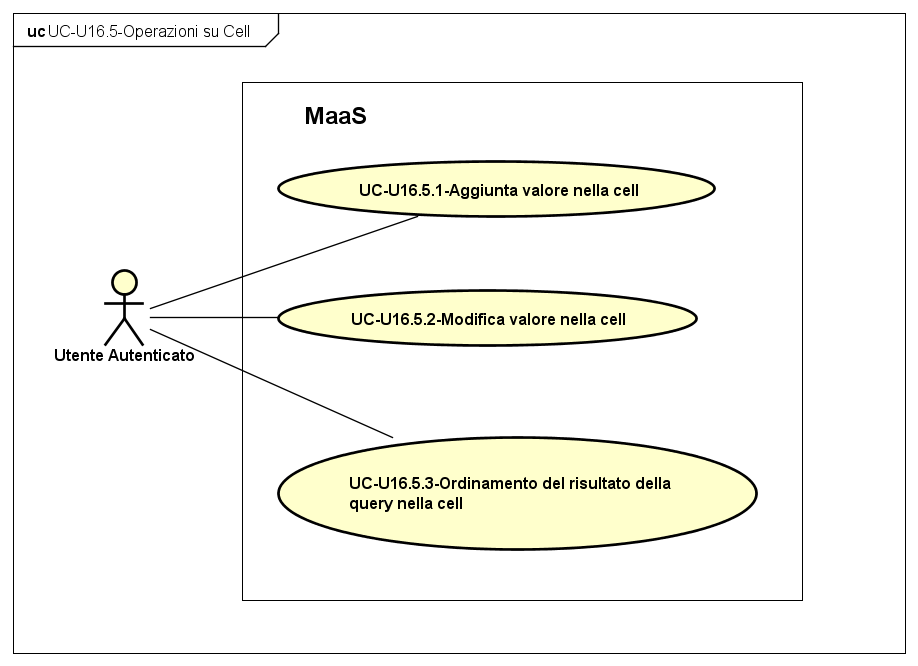
\includegraphics[width=12cm]{res/img/UCUtenti/UCUtenteA/UC-U16.5-Operazioni_su_Cell/UC-U16.5-Operazioni_su_Cell}
      \caption{UC-U16.5 - Operazioni su \glossaryItem{Cell}}
      \end{center} 
    \end{figure}

    %Tabella 
    \begin{center}
      \bgroup
      \def\arraystretch{1.8}     
      \begin{longtable}{  p{3.5cm} | p{8cm} } 
        
        \hline
        \multicolumn{2}{ | c | }{ \cellcolor[gray]{0.9} \textbf{UC-U16.5 - Operazioni su \glossaryItem{Cell}}} \\ 
        \hline
        
        \textbf{Attori Primari} & Utente autenticato \\ 
        \textbf{Scopo e Descrizione} & L'utente autenticato può eseguire le seguenti operazioni dalla pagina \glossaryItem{Cell}: può aggiungere un valore arbitrario, può modificarne uno, può ordinare il valore nella \glossaryItem{Cell} in base all'unico campo della query (scritta in un momento precedente nell'editor) che ha prodotto tale valore. \\ 
        
        \textbf{Precondizioni}  & L'utente autenticato ha visualizzato la pagina \glossaryItem{Cell}. \\ 
        
        \textbf{Postcondizioni} & L'applicazione MaaS ha eseguito le operazioni richieste dall'utente autenticato. \\ 
        \textbf{Scenario principale} & 1. L'utente autenticato aggiunge un valore arbitrario nella \glossaryItem{Cell}. (UC-U16.5.1)
        
2. L'utente autenticato modifica il valore nella \glossaryItem{Cell}. (UC-U16.5.2)

3. L'utente autenticato ordina il valore nella \glossaryItem{Cell}. (UC-U16.5.3) \\
      \end{longtable}
      \egroup
    \end{center}
	
\subsubsection{UC-U16.5.1}

    %Tabella 
    \begin{center}
      \bgroup
      \def\arraystretch{1.8}     
      \begin{longtable}{  p{3.5cm} | p{8cm} } 
        
        \hline
        \multicolumn{2}{ | c | }{ \cellcolor[gray]{0.9} \textbf{UC-U16.5.1 - Aggiunta di un valore nella \glossaryItem{Cell}}} \\ 
        \hline
        
        \textbf{Attori Primari} & Utente autenticato \\ 
        \textbf{Scopo e Descrizione} & L'utente autenticato può aggiungere un valore arbitrario nella \glossaryItem{Cell}.  \\ 
        
        \textbf{Precondizioni}  & L'utente autenticato ha visualizzato la pagina \glossaryItem{Cell}.  \\ 
        
        \textbf{Postcondizioni} & L'utente autenticato ha aggiunto un valore arbitrario nella \glossaryItem{Cell}. \\ 
      \end{longtable}
      \egroup
    \end{center}
    
\subsubsection{UC-U16.5.2}

    %Tabella 
    \begin{center}
      \bgroup
      \def\arraystretch{1.8}     
      \begin{longtable}{  p{3.5cm} | p{8cm} } 
        
        \hline
        \multicolumn{2}{ | c | }{ \cellcolor[gray]{0.9} \textbf{UC-U16.5.2 - Modifica valore \glossaryItem{Cell}}} \\ 
        \hline
        
        \textbf{Attori Primari} & Utente autenticato \\ 
        \textbf{Scopo e Descrizione} & L'utente autenticato può modificare il valore della \glossaryItem{Cell}. \\ 
        
        \textbf{Precondizioni}  & L'utente autenticato ha visualizzato la pagina \glossaryItem{Cell}. \\ 
        
        \textbf{Postcondizioni} & L'utente autenticato ha modificato il valore della \glossaryItem{Cell}. \\ 
      \end{longtable}
      \egroup
    \end{center}
\subsubsection{UC-U16.5.3}

    %Tabella 
    \begin{center}
      \bgroup
      \def\arraystretch{1.8}     
      \begin{longtable}{  p{3.5cm} | p{8cm} } 
        
        \hline
        \multicolumn{2}{ | c | }{ \cellcolor[gray]{0.9} \textbf{UC-U16.5.3 - Ordinamento \glossaryItem{Cell}}} \\ 
        \hline
        
        \textbf{Attori Primari} & Utente autenticato \\ 
        \textbf{Scopo e Descrizione} & L'utente autenticato può ordinare il valore nella \glossaryItem{Cell} in base all'unico campo della query (scritta in un momento precedente nell'editor) che ha prodotto tale valore. \\ 
        
        \textbf{Precondizioni}  & L'utente autenticato ha visualizzato la pagina \glossaryItem{Cell}. \\ 
        
        \textbf{Postcondizioni} & L'utente autenticato ha ordinato il valore della \glossaryItem{Cell}. \\ 
      \end{longtable}
      \egroup
    \end{center}

\subsubsection{UC-U16.6}
 

    \begin{figure}[H]
      \begin{center}
        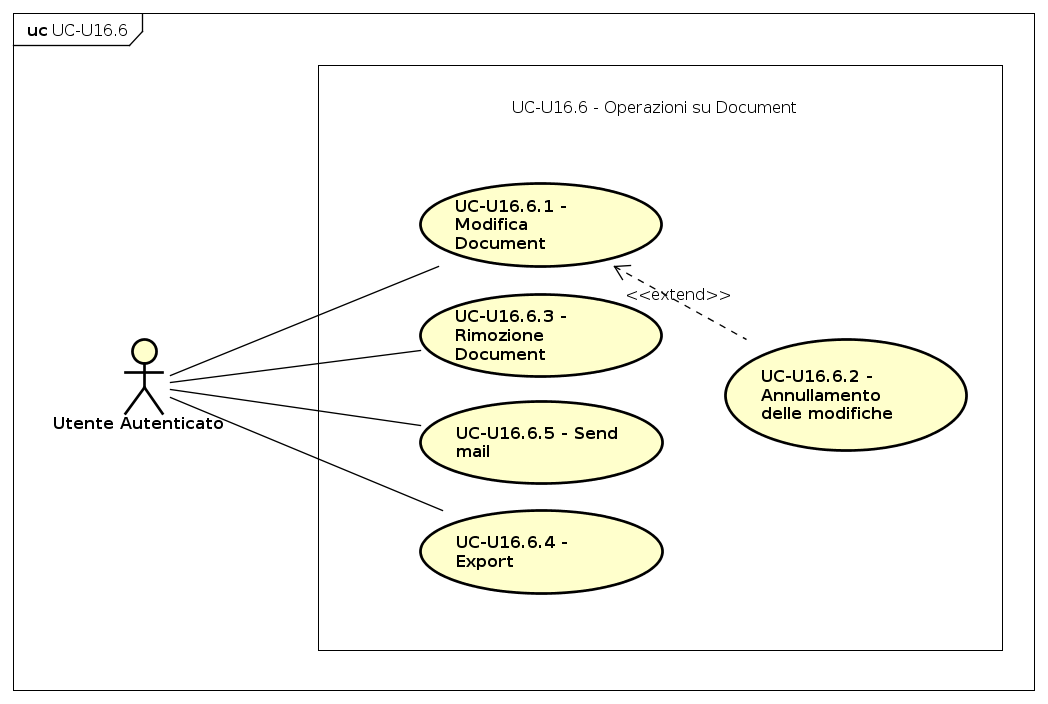
\includegraphics[width=12cm]{res/img/UCUtenti/UCUtenteA/UC-U16.6-Operazioni_su_Document/UC-U16.6}
      \caption{UC-U16.6 - Operazioni su \glossaryItem{Document}}
      \end{center} 
    \end{figure}

    %Tabella 
    \begin{center}
      \bgroup
      \def\arraystretch{1.8}     
      \begin{longtable}{  p{3.5cm} | p{8cm} } 
        
        \hline
        \multicolumn{2}{ | c | }{ \cellcolor[gray]{0.9} \textbf{UC-U16.6 - Operazioni su \glossaryItem{Document}}} \\ 
        \hline
        
        \textbf{Attori Primari} & Utente autenticato \\ 
        \textbf{Scopo e Descrizione} & L'utente autenticato può effettuare le seguenti operazioni sul \textit{Document}: modificarlo, rimuoverlo, eseguire un'operazione di `Export' o di `Send mail'. \\ 
        
        \textbf{Precondizioni}  & L'utente autenticato ha visualizzato la pagina \glossaryItem{Document}. \\ 
        
        \textbf{Postcondizioni} & L'applicazione MaaS ha eseguito le operazioni richieste dall'utente autenticato. \\ 
        \textbf{Scenario principale} & 1. L'utente autenticato modifica un \glossaryItem{Document} (UC-U16.6.1)
        
2. L'utente autenticato rimuove un \glossaryItem{Document} (UC-U16.6.3)

3. L'utente autenticato esporta il \textit{Document} in formato \textit{json} o \textit{csv} (UC-U16.6.4)

4. L'utente autenticato invia una mail a un altro utente (UC-U16.6.5)\\
        \textbf{Estensioni} & 1. L'utente desidera annullare le modifiche apportate a un \glossaryItem{Document} (UC-U16.6.2) \\
      \end{longtable}
      \egroup
    \end{center}
    
\subsubsection{UC-U16.6.1}

    %Tabella 
    \begin{center}
      \bgroup
      \def\arraystretch{1.8}     
      \begin{longtable}{  p{3.5cm} | p{8cm} } 
        
        \hline
        \multicolumn{2}{ | c | }{ \cellcolor[gray]{0.9} \textbf{UC-U16.6.1 - Modifica \glossaryItem{Document}}} \\ 
        \hline
        
        \textbf{Attori Primari} & Utente autenticato \\ 
        \textbf{Scopo e Descrizione} & L'utente autenticato può modificare un \glossaryItem{Document} (modifica il valore di uno dei campi visualizzati nella pagina \glossaryItem{Document} selezionata). \\ 
        
        \textbf{Precondizioni}  & L'utente autenticato ha visualizzato una pagina \glossaryItem{Document} all'interno della quale desidera apportare delle modifiche. \\ 
        
        \textbf{Postcondizioni} & L'applicazione MaaS ha apportato le modifiche richieste dall'utente al \glossaryItem{Document} selezionato. \\ 
      \end{longtable}
      \egroup
    \end{center}
    
\subsubsection{UC-U16.6.2}

    %Tabella 
    \begin{center}
      \bgroup
      \def\arraystretch{1.8}     
      \begin{longtable}{  p{3.5cm} | p{8cm} } 
        
        \hline
        \multicolumn{2}{ | c | }{ \cellcolor[gray]{0.9} \textbf{UC-U16.6.2 - Annullamento delle modifiche di \glossaryItem{Document}}} \\ 
        \hline
        
        \textbf{Attori Primari} & Utente autenticato \\ 
        \textbf{Scopo e Descrizione} & L'utente autenticato può annullare le modifiche precedentemente apportate al \glossaryItem{Document} selezionato. \\ 
        
        \textbf{Precondizioni}  & L'utente autenticato ha apportato delle modifiche a un \glossaryItem{Document}. \\ 
        
        \textbf{Postcondizioni} & Le modifiche apportate dall'utente autenticato al \glossaryItem{Document} selezionato sono state annullate. \\ 
      \end{longtable}
      \egroup
    \end{center}

\subsubsection{UC-U16.6.3}

    %Tabella 
    \begin{center}
      \bgroup
      \def\arraystretch{1.8}     
      \begin{longtable}{  p{3.5cm} | p{8cm} } 
        
        \hline
        \multicolumn{2}{ | c | }{ \cellcolor[gray]{0.9} \textbf{UC-U16.6.3 - Rimozione \glossaryItem{Document}}} \\ 
        \hline
        
        \textbf{Attori Primari} & Utente autenticato \\ 
        \textbf{Scopo e Descrizione} & L'utente autenticato può rimuovere un \glossaryItem{Document} dalla \glossaryItem{Dashboard}. \\ 
        
        \textbf{Precondizioni}  & L'utente autenticato ha visualizzato la pagina \glossaryItem{Document} da rimuovere. \\ 
        
        \textbf{Postcondizioni} & La pagina \glossaryItem{Document} selezionata è stata rimossa. \\ 
      \end{longtable}
      \egroup
    \end{center}
    
\subsubsection{UC-U16.6.4}

    %Tabella 
    \begin{center}
      \bgroup
      \def\arraystretch{1.8}     
      \begin{longtable}{  p{3.5cm} | p{8cm} } 
        
        \hline
        \multicolumn{2}{ | c | }{ \cellcolor[gray]{0.9} \textbf{UC-U16.6.4 - Export di un \glossaryItem{Document}}} \\ 
        \hline
        
        \textbf{Attori Primari} & Utente autenticato \\ 
        \textbf{Scopo e Descrizione} & L'utente autenticato può esportare il \textit{Document} corrente in formato
        \textit{json} o \textit{csv}. \\ 
        
        \textbf{Precondizioni}  & L'utente autenticato ha visualizzato la pagina del \glossaryItem{Document} su cui effettuare le operazioni di `Export' o di `Send email'. \\ 
        
        \textbf{Postcondizioni} & L'applicazione MaaS ha eseguito la richiesta dell'utente. \\ 
      \end{longtable}
      \egroup
    \end{center}
    
\subsubsection{UC-U16.6.5}

    %Tabella 
    \begin{center}
      \bgroup
      \def\arraystretch{1.8}     
      \begin{longtable}{  p{3.5cm} | p{8cm} } 
        
        \hline
        \multicolumn{2}{ | c | }{ \cellcolor[gray]{0.9} \textbf{UC-U16.6.5 - Send Mail da un \glossaryItem{Document}}} \\ 
        \hline
        
        \textbf{Attori Primari} & Utente autenticato \\ 
        \textbf{Scopo e Descrizione} & L'utente autenticato può inviare una mail contenente il \glossaryItem{Document} a un altro utente. \\ 
        
        \textbf{Precondizioni}  & L'utente autenticato ha visualizzato la pagina \glossaryItem{Document} su cui effettuare l'operazione di `Send mail`. \\ 
        
        \textbf{Postcondizioni} & L'applicazione ha inviato la mail con il \glossaryItem{Document} al destinatario segnalato dall'utente. \\ 
      \end{longtable}
      \egroup
    \end{center}


    
\subsubsection{UC-U16.7}
 

    \begin{figure}[H]
      \begin{center}
        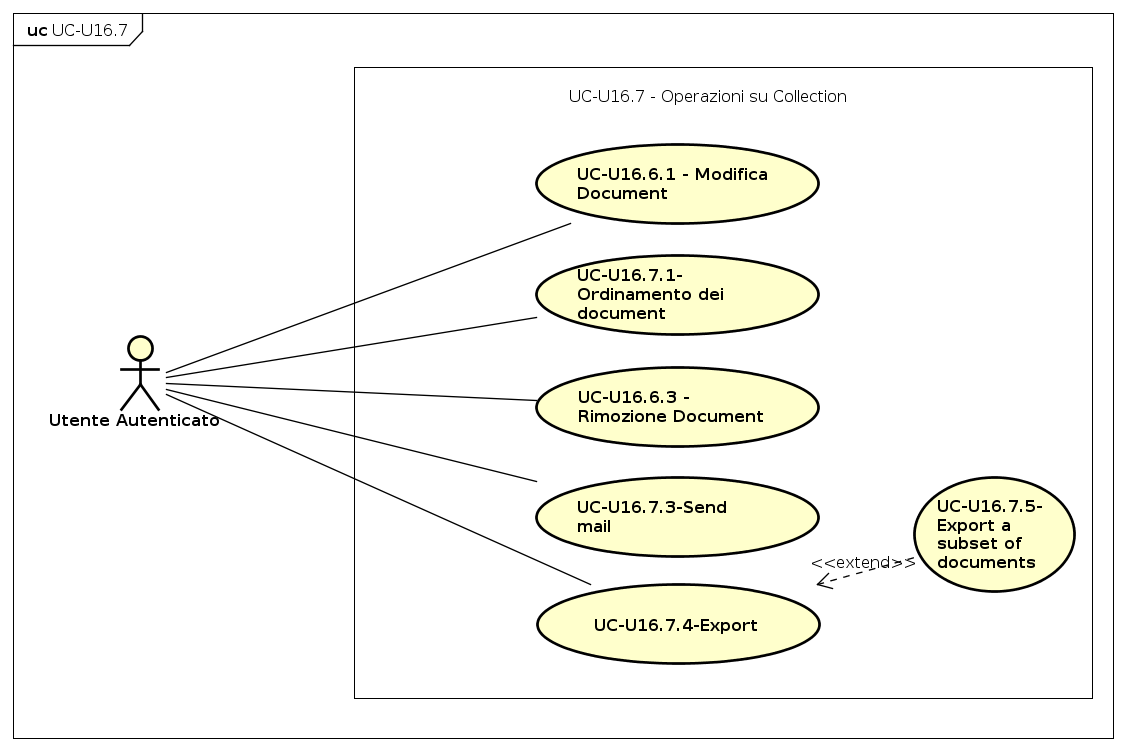
\includegraphics[width=12cm]{res/img/UCUtenti/UCUtenteA/UC-U16.7-Operazioni_su_Collection/UC-U16.7.png}
      \caption{UC-U16.7 - Operazioni su \glossaryItem{Collection}}
      \end{center} 
    \end{figure}

    %Tabella 
    \begin{center}
      \bgroup
      \def\arraystretch{1.8}     
      \begin{longtable}{  p{3.5cm} | p{8cm} } 
        
        \hline
        \multicolumn{2}{ | c | }{ \cellcolor[gray]{0.9} \textbf{UC-U16.7 - Operazioni su \glossaryItem{Collection}}} \\ 
        \hline
        
        \textbf{Attori Primari} & Utente autenticato \\ 
        \textbf{Scopo e Descrizione} & L'utente autenticato può eseguire una delle seguenti operazioni su un pagina \glossaryItem{Collection}: modificare un \glossaryItem{Document}, filtrare i \glossaryItem{Document}, selezionare e visualizzare un sottoinsieme di attributi di un sottoinsieme di \glossaryItem{Document}, rimuovere un \glossaryItem{Document}, eseguire un'azione di default (Export o Send Mail), o un'azione personalizzata. \\ 
        
        \textbf{Precondizioni}  & L'utente autenticato ha visualizzato la pagina \glossaryItem{Collection}. \\ 
        
        \textbf{Postcondizioni} & L'applicazione MaaS ha eseguito le operazioni richieste dall'utente autenticato. \\ 
        \textbf{Scenario principale} & 1. L'utente autenticato può modificare un \glossaryItem{Document} (UC-U16.6.1)

2. L'utente autenticato può ordinare i Documents. (UC-U16.7.1)

3. L'utente autenticato può rimuovere un \glossaryItem{Document}. (UC-U16.6.3)

4. L'utente autenticato può eseguire l'azione di `send mail`. (UC-U16.7.3)

5. L'utente autenticato può eseguire l'azione di `export` su un singolo \glossaryItem{Document}. (UC-U16.6.4) \\

        \textbf{Estensioni} & 1. L'utente può selezionare solo un sottoinsieme di elementi ed esportarli in formato json o csv (UC-U16.7.4) \\
      \end{longtable}
      \egroup
    \end{center}
    
\subsubsection{UC-U16.7.1}

    %Tabella 
    \begin{center}
      \bgroup
      \def\arraystretch{1.8}     
      \begin{longtable}{  p{3.5cm} | p{8cm} } 
        
        \hline
        \multicolumn{2}{ | c | }{ \cellcolor[gray]{0.9} \textbf{UC-U16.7.1 - Ordina \glossaryItem{Document}}} \\ 
        \hline
        
        \textbf{Attori Primari} & Utente autenticato \\ 
        \textbf{Scopo e Descrizione} & L'utente autenticato può decidere di ordinare i \glossaryItem{Document} della \glossaryItem{Collection} in base a uno dei loro attributi. \\ 
        
        \textbf{Precondizioni}  & L'utente autenticato ha visualizzato la pagina \glossaryItem{Collection}. \\ 
        
        \textbf{Postcondizioni} & L'applicazione ha ordinato i \glossaryItem{Document} secondo l'ordine indicato dall'utente. \\ 
      \end{longtable}
      \egroup
    \end{center}
    
      

    
\subsubsection{UC-U16.7.3}

    %Tabella 
    \begin{center}
      \bgroup
      \def\arraystretch{1.8}     
      \begin{longtable}{  p{3.5cm} | p{8cm} } 
        
        \hline
        \multicolumn{2}{ | c | }{ \cellcolor[gray]{0.9} \textbf{UC-U16.7.3 - Send mail da una \glossaryItem{Collection}}} \\ 
        \hline
        
        \textbf{Attori Primari} & Utente autenticato \\ 
        \textbf{Scopo e Descrizione} & L'utente autenticato può inviare una email contenente i Documents selezionati a un altro utente. \\ 
        
        \textbf{Precondizioni}  & L'utente ha visualizzato la pagina \glossaryItem{Collection}. \\ 
        
        \textbf{Postcondizioni} & L'applicazione ha inviato la mail con i Documents selezionati al destinatario indicato dall'utente. \\ 
      \end{longtable}
      \egroup
     \end{center}
      
\subsubsection{UC-U16.7.4}

    %Tabella 
    \begin{center}
      \bgroup
      \def\arraystretch{1.8}     
      \begin{longtable}{  p{3.5cm} | p{8cm} } 
        
        \hline
        \multicolumn{2}{ | c | }{ \cellcolor[gray]{0.9} \textbf{UC-U16.7.4 - Export di una \glossaryItem{Collection}}} \\ 
        \hline
        
        \textbf{Attori Primari} & Utente autenticato \\ 
        \textbf{Scopo e Descrizione} & L'utente autenticato può esportare i Documents selezionati da una \glossaryItem{Collection} in formato json o csv. \\ 
        
        \textbf{Precondizioni}  & L'utente autenticato ha selezionato i documenti da esportare e il formato di file con cui intende scaricarli. \\ 
        
        \textbf{Postcondizioni} & L'applicazione ha eseguito creato il file con i dati selezionati scaricabile nel formato scelto dall'utente. \\ 
      \end{longtable}
      \egroup
    \end{center}
    
    
\subsubsection{UC-U17}
      
        %Tabella 
        \begin{center}
          \bgroup
          \def\arraystretch{1.8}     
          \begin{longtable}{  p{3.5cm} | p{8cm} } 
            
            \hline
            \multicolumn{2}{ | c | }{ \cellcolor[gray]{0.9} \textbf{UC-U17 - Logout}} \\ 
            \hline
            
            \textbf{Attori Primari} & Utente autenticato \\ 
            \textbf{Scopo e Descrizione} & L’utente autenticato vuole effettuare il logout dall'applicazione.\\ 
            
            \textbf{Precondizioni}  & L'utente autenticato è loggato con le sue credenziali. \\ 
            
            \textbf{Postcondizioni} & L'utente autenticato visualizza un messaggio di avvenuto logout e viene disconnesso. \\ 
          \end{longtable}
          \egroup
        \end{center}
\newpage

